%!TEX root = ../Hardtung_BA_SoSe20.tex

\section{Introduction}
\label{sec:introduction}

\gls{origami} is the Japanese art of folding paper into models of animals, people or other objects. Folding such models can be a complex task, so in order to make origami more accessible, a system of folding instructions was developed. The diagramming system developed by Akira Yoshizawa was first published in the book \emph{Atarashi origami geijutsu} in 1954 \cite{Yoshizawa}. Yoshizawa's origami notation introduced a set of symbols and arrows to explain the different folding actions. After further development by Sam Randlett and Robert Harbin this set of origami symbols became the international standard \cite{origamiHistoryWu} \cite{origamiHistoryK}.
By creating these drawings for each folding step, even origami beginners could fold models. These origami diagrams (see Figure \ref{fig:craneDiagram}) have to be accurate representations of the paper for every folding step, in order to unambiguously explain how to fold the model. Every flap, crease and edge has to be drawn, which makes the process slow and especially error-prone for complex models. While for example the crane model in Figure \ref{fig:craneDiagram} can be folded in 17 steps, more complex models can take hundreds of steps to complete. 

\begin{figure}[htbp]
	\centering
	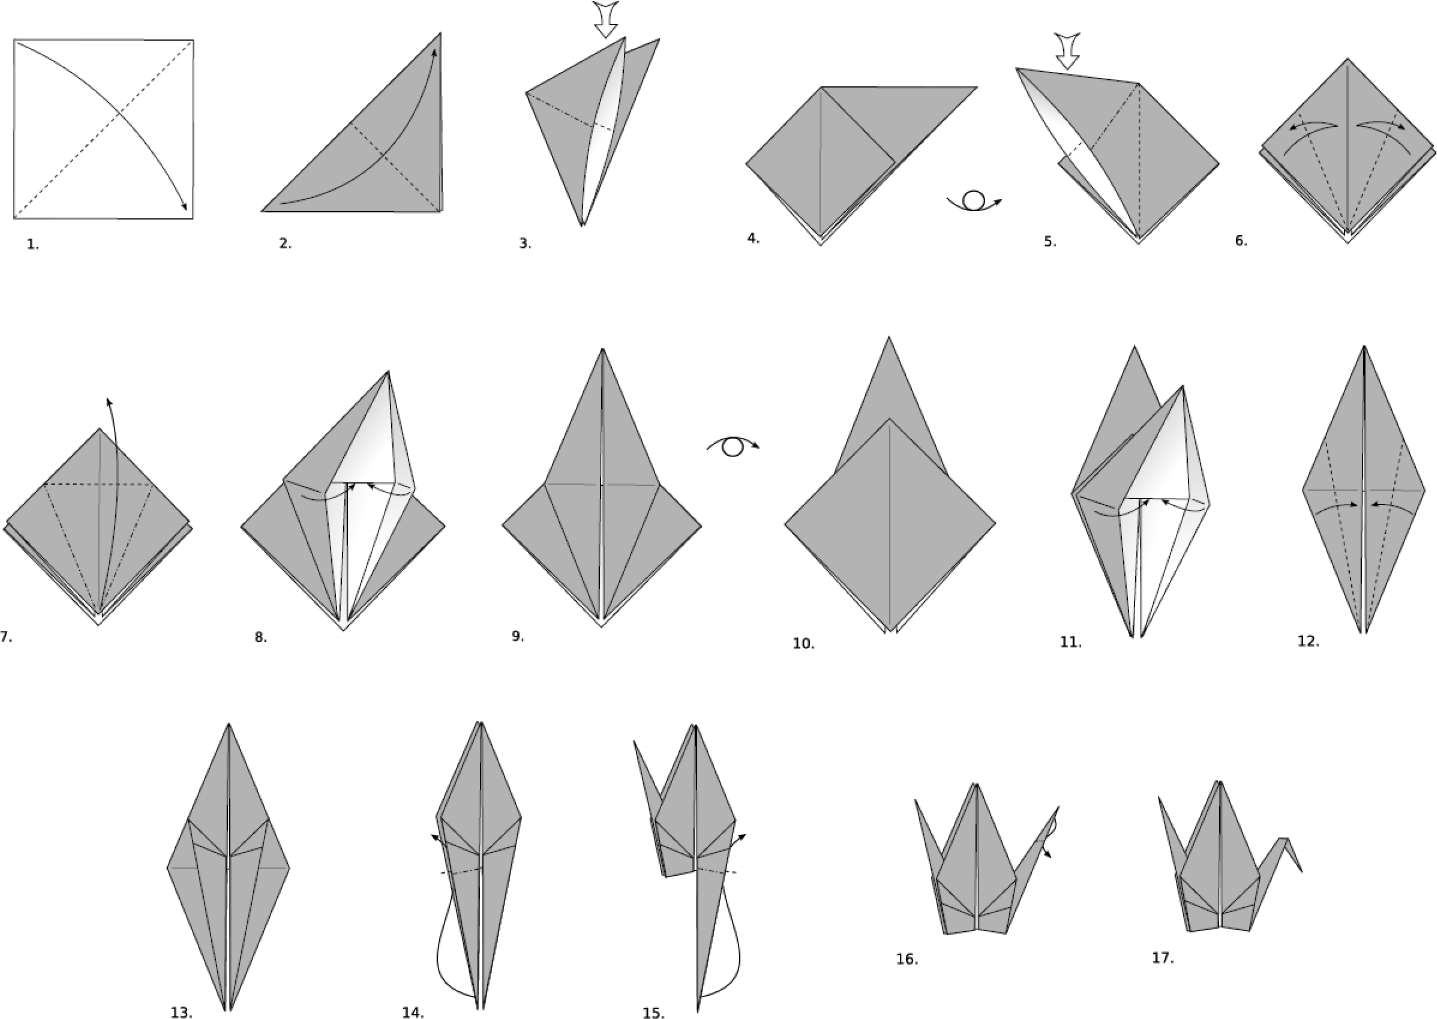
\includegraphics[width=\textwidth]{Crane}
	\caption[Crane Diagram]{Crane Diagram - [Andrew Hudson, 2011 \cite{Hudson}]}
	\label{fig:craneDiagram}
\end{figure}

\noindent In order to help artists during the creation process for origami diagrams, the \gls{origrammer} \cite{origrammer} was developed.

The Origrammer is a desktop application, developed by the author, which offers specific features for creating such diagrams. This program simulates, how an origami artist would create diagrams by hand. Lines, arrows, and symbols can be placed and new diagram steps can be created. Additionally, helping features are included to speed up the diagramming process as a whole. A more detailed overview and explanation of the Origrammer can be found in Section \ref{sec:origrammer}.

This Bachelor Thesis now aims to evaluate the current state of this program and to develop it further to improve usability, efficiency and effectivity. This thesis will start with a short summary on how the Origrammer works and what a typical workflow looks like. Afterwards, an evaluation has to be carried out, in order to get a sense of the current state of this program. Flaws and missing features have to be explicitly defined, so that a plan can be created on how to further improve the Origrammer.

As the evaluation will potentially find a multitude of different types of flaws and problems, a specific focus has to be defined. In case of this thesis, the main goal is to maximise the speed of creating origami diagrams, while also offering a usable user interface with which also novizes can work with ease. This target was set with the original plan of the Origrammer in mind:

\begin{center}
\enquote{\emph{The goal for this project is to develop a desktop application that implements features specifically for the origami diagramming process. The standardized symbols and overall notations have to be included and the program \textbf{has to offer functions that increase the efficiency of creating diagrams}.}} (Hardtung, 2020, p.5 \cite{origrammer})
\end{center}

\noindent Then after evaluating and collecting potential improvements, a more detailed plan can be created on how to actually implement these changes. Although not all potential improvements can be implemented within the scope of this thesis, all found flaws should be categorized and documented, which can help further development in the future.